% ARTICLE 2 ----
% This is just here so I know exactly what I'm looking at in Rstudio when messing with stuff.
% Options for packages loaded elsewhere
\PassOptionsToPackage{unicode}{hyperref}
\PassOptionsToPackage{hyphens}{url}
%
\documentclass[
  11pt,
]{article}
\usepackage{lmodern}
\usepackage{amssymb,amsmath}
\usepackage{ifxetex,ifluatex}
\ifnum 0\ifxetex 1\fi\ifluatex 1\fi=0 % if pdftex
  \usepackage[T1]{fontenc}
  \usepackage[utf8]{inputenc}
  \usepackage{textcomp} % provide euro and other symbols
\else % if luatex or xetex
  \usepackage{unicode-math}
  \defaultfontfeatures{Scale=MatchLowercase}
  \defaultfontfeatures[\rmfamily]{Ligatures=TeX,Scale=1}
\fi
% Use upquote if available, for straight quotes in verbatim environments
\IfFileExists{upquote.sty}{\usepackage{upquote}}{}
\IfFileExists{microtype.sty}{% use microtype if available
  \usepackage[]{microtype}
  \UseMicrotypeSet[protrusion]{basicmath} % disable protrusion for tt fonts
}{}
\makeatletter
\@ifundefined{KOMAClassName}{% if non-KOMA class
  \IfFileExists{parskip.sty}{%
    \usepackage{parskip}
  }{% else
    \setlength{\parindent}{0pt}
    \setlength{\parskip}{6pt plus 2pt minus 1pt}
    }
}{% if KOMA class
  \KOMAoptions{parskip=half}}
\makeatother
\usepackage{xcolor}
\IfFileExists{xurl.sty}{\usepackage{xurl}}{} % add URL line breaks if available
\urlstyle{same} % disable monospaced font for URLs
\usepackage[margin=1in]{geometry}
\usepackage{graphicx}
\makeatletter
\def\maxwidth{\ifdim\Gin@nat@width>\linewidth\linewidth\else\Gin@nat@width\fi}
\def\maxheight{\ifdim\Gin@nat@height>\textheight\textheight\else\Gin@nat@height\fi}
\makeatother
% Scale images if necessary, so that they will not overflow the page
% margins by default, and it is still possible to overwrite the defaults
% using explicit options in \includegraphics[width, height, ...]{}
\setkeys{Gin}{width=\maxwidth,height=\maxheight,keepaspectratio}
% Set default figure placement to htbp
\makeatletter
\def\fps@figure{htbp}
\makeatother
\setlength{\emergencystretch}{3em} % prevent overfull lines
\providecommand{\tightlist}{%
  \setlength{\itemsep}{0pt}\setlength{\parskip}{0pt}}
\setcounter{secnumdepth}{5}

\ifluatex
  \usepackage{selnolig}  % disable illegal ligatures
\fi
\newlength{\cslhangindent}
\setlength{\cslhangindent}{1.5em}
\newlength{\csllabelwidth}
\setlength{\csllabelwidth}{3em}
\newenvironment{CSLReferences}[2] % #1 hanging-ident, #2 entry spacing
 {% don't indent paragraphs
  \setlength{\parindent}{0pt}
  % turn on hanging indent if param 1 is 1
  \ifodd #1 \everypar{\setlength{\hangindent}{\cslhangindent}}\ignorespaces\fi
  % set entry spacing
  \ifnum #2 > 0
  \setlength{\parskip}{#2\baselineskip}
  \fi
 }%
 {}
\usepackage{calc}
\newcommand{\CSLBlock}[1]{#1\hfill\break}
\newcommand{\CSLLeftMargin}[1]{\parbox[t]{\csllabelwidth}{#1}}
\newcommand{\CSLRightInline}[1]{\parbox[t]{\linewidth - \csllabelwidth}{#1}\break}
\newcommand{\CSLIndent}[1]{\hspace{\cslhangindent}#1}


\title{Disagreement and dissent on a bench: a quantitative empirical
analysis of the Czech Constitutional Court\thanks{Replication files are
available on the author's Github account
(\url{https://github.com/stepanpaulik/apex_courts_dataset/}).
\textbf{Current version}: February 03, 2024}}
\author{true \and true}
\date{February 03, 2024}

% Jesus, okay, everything above this comment is default Pandoc LaTeX template. -----
% ----------------------------------------------------------------------------------
% I think I had assumed beamer and LaTex were somehow different templates.


\usepackage{kantlipsum}

\usepackage{abstract}
\renewcommand{\abstractname}{}    % clear the title
\renewcommand{\absnamepos}{empty} % originally center

\renewenvironment{abstract}
 {{%
    \setlength{\leftmargin}{0mm}
    \setlength{\rightmargin}{\leftmargin}%
  }%
  \relax}
 {\endlist}

\makeatletter
\def\@maketitle{%
  \newpage
%  \null
%  \vskip 2em%
%  \begin{center}%
  \let \footnote \thanks
      {\fontsize{18}{20}\selectfont\raggedright  \setlength{\parindent}{0pt} \@title \par}
    }
%\fi
\makeatother


\title{Disagreement and dissent on a bench: a quantitative empirical
analysis of the Czech Constitutional Court\thanks{Replication files are
available on the author's Github account
(\url{https://github.com/stepanpaulik/apex_courts_dataset/}).
\textbf{Current version}: February 03, 2024}  }

\date{}

\usepackage{titlesec}

% 
\titleformat*{\section}{\large\bfseries}
\titleformat*{\subsection}{\normalsize\itshape} % \small\uppercase
\titleformat*{\subsubsection}{\normalsize\itshape}
\titleformat*{\paragraph}{\normalsize\itshape}
\titleformat*{\subparagraph}{\normalsize\itshape}

% add some other packages ----------

% \usepackage{multicol}
% This should regulate where figures float
% See: https://tex.stackexchange.com/questions/2275/keeping-tables-figures-close-to-where-they-are-mentioned
\usepackage[section]{placeins}



\makeatletter
\@ifpackageloaded{hyperref}{}{%
\ifxetex
  \PassOptionsToPackage{hyphens}{url}\usepackage[setpagesize=false, % page size defined by xetex
              unicode=false, % unicode breaks when used with xetex
              xetex]{hyperref}
\else
  \PassOptionsToPackage{hyphens}{url}\usepackage[draft,unicode=true]{hyperref}
\fi
}

\@ifpackageloaded{color}{
    \PassOptionsToPackage{usenames,dvipsnames}{color}
}{%
    \usepackage[usenames,dvipsnames]{color}
}
\makeatother
\hypersetup{breaklinks=true,
            bookmarks=true,
            pdfauthor={Štěpán Paulík (Humboldt Universität zu Berlin,
\href{mailto:stepan.paulik.1@hu-berlin.de}{\nolinkurl{stepan.paulik.1@hu-berlin.de}}) and Gor
Vartazaryan (Charles University,
\href{mailto:gorike2000@gmail.com}{\nolinkurl{gorike2000@gmail.com}})},
             pdfkeywords = {empirical legal research, courts, dissents,
judicial behavior, political science, regression analysis},
            pdftitle={Disagreement and dissent on a bench: a
quantitative empirical analysis of the Czech Constitutional Court},
            colorlinks=true,
            citecolor=blue,
            urlcolor=blue,
            linkcolor=magenta,
            pdfborder={0 0 0}}
\urlstyle{same}  % don't use monospace font for urls

% Add an option for endnotes. -----



% This will better treat References as a section when using natbib
% https://tex.stackexchange.com/questions/49962/bibliography-title-fontsize-problem-with-bibtex-and-the-natbib-package

% set default figure placement to htbp
\makeatletter
\def\fps@figure{htbp}
\makeatother



\usepackage{longtable}
\LTcapwidth=.95\textwidth
\linespread{1.05}
\usepackage{hyperref}
\usepackage{float}
\usepackage{booktabs}
\usepackage{longtable}
\usepackage{array}
\usepackage{multirow}
\usepackage{wrapfig}
\usepackage{float}
\usepackage{colortbl}
\usepackage{pdflscape}
\usepackage{tabu}
\usepackage{threeparttable}
\usepackage{threeparttablex}
\usepackage[normalem]{ulem}
\usepackage{makecell}
\usepackage{xcolor}
\usepackage{siunitx}

  \newcolumntype{d}{S[
    input-open-uncertainty=,
    input-close-uncertainty=,
    parse-numbers = false,
    table-align-text-pre=false,
    table-align-text-post=false
  ]}
  

\newtheorem{hypothesis}{Hypothesis}

\usepackage{setspace}

% trick for moving figures to back of document
% really wish we'd knock this shit off with moving tables/figures to back of document
% but, alas...

% 
% Optional code chunks ------
% SOURCE: https://stackoverflow.com/questions/50702942/does-rmarkdown-allow-captions-and-references-for-code-chunks



\begin{document}

% \textsf{\textbf{This is sans-serif bold text.}}
% \textbf{\textsf{This is bold sans-serif text.}}


% \maketitle

{% \usefont{T1}{pnc}{m}{n}
\setlength{\parindent}{0pt}
\thispagestyle{plain}
{%\fontsize{18}{20}\selectfont\raggedright
\maketitle  % title \par

}




{
   \vskip 13.5pt\relax \normalsize\fontsize{11}{12}
   \MakeUppercase{Štěpán Paulík}, \small{Humboldt Universität zu Berlin,
\href{mailto:stepan.paulik.1@hu-berlin.de}{\nolinkurl{stepan.paulik.1@hu-berlin.de}}}   \par \vskip -3.5pt \MakeUppercase{Gor
Vartazaryan}, \small{Charles University,
\href{mailto:gorike2000@gmail.com}{\nolinkurl{gorike2000@gmail.com}}}   

}

}








\begin{abstract}

%    \hbox{\vrule height .2pt width 39.14pc}

    \vskip 8.5pt % \small

\noindent \small{XXX}


\vskip 8.5pt \noindent \emph{Keywords}: empirical legal research,
courts, dissents, judicial behavior, political science, regression
analysis \par

%    \hbox{\vrule height .2pt width 39.14pc}



\end{abstract}


\vskip -8.5pt

{
\hypersetup{linkcolor=black}
\setcounter{tocdepth}{2}
\tableofcontents
}

 % removetitleabstract

{
\setcounter{tocdepth}{2}
\tableofcontents
}

\setlength{\parindent}{16pt}
\setlength{\parskip}{0pt}

% We'll put doublespacing here
\doublespacing
% Remember to cut it out later before bib
\hypertarget{introduction}{%
\section{Introduction}\label{introduction}}

Empirical legal research has been slowly but surely finding it's outside
the predominant US context. Historically though most of the empirical
studies have been conducted in the US, especially the Supreme Court,
context (such as
\protect\hyperlink{ref-boydUntanglingCausalEffects2010}{Boyd, Epstein,
and Martin 2010};
\protect\hyperlink{ref-carrubbaWhoControlsContent2012}{Carrubba et al.
2012}; \protect\hyperlink{ref-epsteinWhyWhenJudges2011}{Epstein, Landes,
and Posner 2011}). We now know that judgments are what judges had for a
breakfast. Put less pompously, there are many theories and approaches
for explanation of judicial behavior
(\protect\hyperlink{ref-posnerHowJudgesThink2010}{Posner 2010}). What we
do not know is the extent to which these theories and explanations carry
over to other legal systems and context.

Although it has been traditionally espoused that there has been a divide
between the empirically oriented US legal scholarship, stemming from a
different perception of the role of courts and judges, and the rest of
the world (\protect\hyperlink{ref-hamannGermanFederalCourts2019}{Hamann
2019, 416}). Therein the judges empirically researched whether and to
what extent they behave as for example political
(\protect\hyperlink{ref-carrubbaWhoControlsContent2012}{Carrubba et al.
2012}; \protect\hyperlink{ref-clarkLocatingSupremeCourt2010}{Clark and
Lauderdale 2010};
\protect\hyperlink{ref-epsteinChoicesJusticesMake1997}{Epstein and
Knight 1997};
\protect\hyperlink{ref-lauderdaleScalingPoliticallyMeaningful2014}{Lauderdale
and Clark 2014};
\protect\hyperlink{ref-sunsteinAreJudgesPolitical2006}{Sunstein et al.
2006}) or strategic
(\protect\hyperlink{ref-cameronChapterWhatJudges2017}{Cameron and
Kornhauser 2017};
\protect\hyperlink{ref-clarkEstimatingEffectLeisure2018}{Clark, Engst,
and Staton 2018};
\protect\hyperlink{ref-epsteinWhyWhenJudges2011}{Epstein, Landes, and
Posner 2011};
\protect\hyperlink{ref-epsteinStrategicRevolutionJudicial2000}{Epstein
and Knight 2000};
\protect\hyperlink{ref-kornhauserModelingCollegialCourts1992}{Kornhauser
1992b},
\protect\hyperlink{ref-kornhauserModelingCollegialCourts1992a}{1992a};
\protect\hyperlink{ref-posnerWhatJudgesJustices1993}{Posner 1993},
\protect\hyperlink{ref-posnerHowJudgesThink2010}{2010};
\protect\hyperlink{ref-rousseyOverburdenedJudges2018}{Roussey and
Soubeyran 2018}) actors.

In contrast to, especially in European legal systems, such as the one at
hand - Czechia, judges have been perceived as ``proclaimers of law'' and
the law handed down by them
(\protect\hyperlink{ref-hamannGermanFederalCourts2019}{Hamann 2019,
417}). Such a view had hindered empirical legal research in Europe. The
lack of empirical legal research can be partially blamed on lack of high
quality data, a prerequisite for any quantitative empirical research. At
least so the story goes until recently. The interest in empirical legal
studies has picked up in the last years across the whole continent,
including studies on plethora of topics within Germany
(\protect\hyperlink{ref-arnoldScalingCourtDecisions2023}{Arnold, Engst,
and Gschwend 2023};
\protect\hyperlink{ref-coupetteQuantitativeRechtswissenschaft2018}{Coupette
and Fleckner 2018};
\protect\hyperlink{ref-engstEinflussParteinaheAuf2017}{Engst et al.
2017};
\protect\hyperlink{ref-wittigOccurrenceSeparateOpinions2016}{Wittig
2016}), Spain and Portugal
(\protect\hyperlink{ref-hanrettyDissentIberiaIdeal2012}{Hanretty 2012}),
the UK
(\protect\hyperlink{ref-hanrettyCourtSpecialistsJudicial2020}{Hanretty
2020}) or the EU institutions
(\protect\hyperlink{ref-bielenBacklogsLitigationRates2018}{Bielen et al.
2018}; \protect\hyperlink{ref-brekkeThatOrderHow2023}{Brekke, Naurin, et
al. 2023}; \protect\hyperlink{ref-fjelstulHowChamberSystem2023}{Fjelstul
2023}, \protect\hyperlink{ref-fjelstulEvolutionEuropeanUnion2019}{2019};
\protect\hyperlink{ref-fjelstulTimelyAdministrationJustice2022}{Fjelstul,
Gabel, and Carrubba 2022}).

In our article, we set out to conduct an empirical research into the
circumstances of disagreement on a court bench, we empirically research
the circumstances of disagreement among the judges of the Czech
Constitutional Court (``CCC'') and we attempt to square the perception
of judges as rational-economic beings
(\protect\hyperlink{ref-epsteinWhyWhenJudges2011}{Epstein, Landes, and
Posner 2011};
\protect\hyperlink{ref-epsteinStrategicRevolutionJudicial2000}{Epstein
and Knight 2000}), the identification-disagreement model
(\protect\hyperlink{ref-wittigOccurrenceSeparateOpinions2016}{Wittig
2016}), and our empirical findings.

We find that\ldots{}

Our article proceeds as follows. We start out with a theory. We explain
the main differences between the expectations based on the theory in the
CCC context in comparison to the SCOTUS context and based on that we
draw the hypotheses for the empirical part. We briefly explain the
choice of our broad methodological framework: the Bayesian statistics.
We proceed to test the hypotheses in empirical part divided into
sections one per each hypothesis. We discuss the pitfalls of our
research and potential room for improvement afterwards. Lastly, we
conclude with a summary of our findings.

\hypertarget{theory}{%
\section{Theory}\label{theory}}

\hypertarget{overview-of-accounts-of-judicial-decision-making}{%
\subsection{Overview of Accounts of Judicial-Decision
Making}\label{overview-of-accounts-of-judicial-decision-making}}

In general, there are multiple accounts of judicial decision-making
process. At first, judges were perceived as deciding simply by means of
law. Over time, the perception of judges changed The attitudinal
accounts posited that judges are policy oriented. In other words, judges
follow their own ideas and preferences when deciding cases. A lot of
research has been conducted on whether, how and to what extent do judges
indeed seek to advance the policies they desire
(\protect\hyperlink{ref-berdejoElectoralCyclesUS2017}{Berdejó and Chen
2017}; \protect\hyperlink{ref-clarkLocatingSupremeCourt2010}{Clark and
Lauderdale 2010};
\protect\hyperlink{ref-dworkinPoliticalJudgesRule1980}{Dworkin 1980};
\protect\hyperlink{ref-kastellecEmpiricallyEvaluatingCountermajoritarian2016}{Kastellec
2016}; \protect\hyperlink{ref-moyerJudicialInnovationSexual2012}{Moyer
and Tankersley 2012}).

However, as of recently, the perspective on judges has shifted. Judges
are now allegedly strategic and rational actors. One of the early
pioneers of this approach Posner
(\protect\hyperlink{ref-posnerWhatJudgesJustices1993}{1993}) presents a
simple model of judicial utility as function mainly of income, leisure
and judicial voting. Further research followed the Posner mode and
presented alternative models of judicial utility (based on economic
psychology \protect\hyperlink{ref-foxallWhatJudgesMaximize2004}{Foxall
2004}). Replacing the policy oriented approaches, which hold judges to
pursue political policy oriented goals, researchers now focus more on
their self-interest in terms of career progression , higher income, more
leisure, or lesser workload
(\protect\hyperlink{ref-epsteinStrategicRevolutionJudicial2000}{Epstein
and Knight 2000}). For example, Clark, Engst, and Staton
(\protect\hyperlink{ref-clarkEstimatingEffectLeisure2018}{2018}) have in
a quasi-experimental research design found that judges have preferences
regarding their leisure, which then impacts their performance. Brekke,
Naurin, et al. (\protect\hyperlink{ref-brekkeThatOrderHow2023}{2023})
found that the CJEU justices take into account their workload when
issuing orders.

\hypertarget{accounts-of-dissenting-behavior}{%
\subsection{Accounts of Dissenting
Behavior}\label{accounts-of-dissenting-behavior}}

In their empirical study on dissenting behavior on the Supreme Court of
the USA (``SCOTUS''), the proponents of the strategic account Epstein,
Landes, and Posner
(\protect\hyperlink{ref-epsteinWhyWhenJudges2011}{2011}) base their
theory of dissents on the strategic-economic framework of
self-interested strategically motivated judges. They presume that
judges' ``leisure preferences, or, equivalently, effort aversion, which
they trade off against their desire to have a good reputation and to
express their legal and policy beliefs and preferences (and by doing so
perhaps influence law and policy) by their vote, and by the judicial
opinion explaining their vote, in the cases they hear.'' The benefits of
a dissenting opinion are the potential to undermine the majority opinion
when the dissent is influential and the enhanced reputation that the
judge enjoys. The dissenting opinion may be cited in the future by other
judges or publicly analysed by legal scholars.

The theories they presume and hypotheses they test rest on this
framework: in the policy-oriented framework, it would not make sense to
expect judges to dissent less as their workload increases. They would
still seek a way to advance their political agenda and research has
shown that dissenting opinions usually correspond to exactly just that
(\protect\hyperlink{ref-clarkLocatingSupremeCourt2010}{Clark and
Lauderdale 2010}). However, in the strategic account, the higher the
workload of a judge, the more pressing the effort costs of a dissent.
Similarly, if a dissenting opinion imputes costs on the majority, we can
theoretically expect it to respond to the dissent with a more thorough
or detailed argumentation in the majority opinion.

Wittig
(\protect\hyperlink{ref-wittigOccurrenceSeparateOpinions2016}{2016}) in
her dissertation thesis summarizes the potential motivations for judges
to attach a separate opinion and, thus, to acquire additional costs: (1)
potential of impacting future caselaw, (2) moral obligation to distance
oneself from a decision that contradicts her values, (3) to convey
certain image about oneself. These motivations also largely rely on the
self-perceived stance towards separate opinions in general. The
proponents of separate opinions view dissenting positively based on the
separate opinions being able to enrich the legal debate, being a sign of
judicial independence, increasing the legitimacy of any given decision
for it makes the decision more accurate of the real discussion behind
it. The opponents of separate opinions mainly argue that showing the
inability to speak in one voice undermines a court's legitimacy or the
reputation of the dissenting judge. Moreover, judges seeking the
appreciation from the general public or legal community may act in their
personal interests instead of in the court's interests. Lastly, separate
opinions come at collegiality costs and may harm the mutual
relationships of judges.

Wittig makes a sharp cut from the accounts coming mainly from the US,
more specifically from the research on SCOTUS, and comes up with a model
of separate opinions much better suited for the civil law context of the
CCC, the identification-disagreement model. Wittig argues that the
traditional all have limited explanatory power as such and also do not
fit within the civil law context, as judges therein are deciding in a
different context, bound by different procedural rules, and, thus, given
differing, sometimes broader, sometimes more limited, avenues to give
way to their preferences or strategic considerations. We now discuss the
identification-disagreement model in more detail.

\hypertarget{the-identification-disagreement-model-of-dissenting-behavior}{%
\subsection{The Identification-Disagreement Model of Dissenting
Behavior}\label{the-identification-disagreement-model-of-dissenting-behavior}}

Wittig introduces a non-formal model of separate opinions, the
identification-disagreement model. Wittig amalgamates all the previously
introduced potential motivations of judges for writing separate opinions
into one cohesive and comprehensive model. We build on the
identification-disagreement model theoretically and we use it to
generate hypotheses for the CCC.

The model is made up of two dimensions. The first dimensions of the
model covers the disagreement level. The second dimension concerns the
judges' stance and degree of self-identification of their role as a
judge, Wittig terms this as a \emph{norm of consensus}. Separate
opinions are then ``a function of a judge's identification with the norm
of consensus and the level of disagreement of judges
(\protect\hyperlink{ref-wittigOccurrenceSeparateOpinions2016}{Wittig
2016, 74--75}).

\hypertarget{the-norm-of-consensus}{%
\subsubsection{The norm of consensus}\label{the-norm-of-consensus}}

Calderia and Zorn
(\protect\hyperlink{ref-calderiaTimeConsensualNorms1998}{1998}),
p.~876-877 define a norm as ``a long-run equilibrium outcome, which
underpins the interaction between individuals and reflects common
understandings as to what is acceptable behavior in given
circumstances.'' The norm of consensus in turn defines the level of
dissent that is acceptable at any given court
(\protect\hyperlink{ref-narayanConsensualNormHigh2005}{Narayan and Smyth
2005};
\protect\hyperlink{ref-wittigOccurrenceSeparateOpinions2016}{Wittig
2016, 75}.). Wittig's argument is two-fold. First, in civil law
traditions unlike its US counterpart, the prevailing notion of the norm
of consensus is that a court should not display disagreement. Second,
the extent of adherence to the norm varies among judges,\footnote{We
  conducted interviews with the justices of the third term of the CCC.
  Many of them more or less directly confirmed that they either share
  this self-perception to a highly varying degree.} depending on how
they weight the costs and benefits they receive from following it
(\protect\hyperlink{ref-wittigOccurrenceSeparateOpinions2016}{Wittig
2016, 75}.).

A disonance between a proposed outcome for a case and any given judge's
preferences are eventually bound to happen. In such a case, the judge
can either express their sincere preferences by writing a separate
opinion or they can adapt their behavior according to the norm of
consensus and suppress the expression of her preferences. The second
route has also been termed \emph{dissent aversion} and theoretically
fleshed out by Epstein, Landes, and Posner
(\protect\hyperlink{ref-epsteinWhyWhenJudges2011}{2011}). The decision
of judge faced with such a conflict whether to attach a separate opinion
or whether to avert their dissent is then a function of multiple
potential utilities.

Wittig draws up three types of utility that dictate various levels of
the adherence to the norm of consensus. Firstly, the intrinsic utility
is maximazed whenever a judge behaves in accordance with their true
values and opinions, setting aside their strategic or political
considerations. Secondly, expressive utility is harnessed when one
displays individuality and counters the notion of conformism. Thirdly,
the reputational utility arises when one adjusts their publicly
displayed preferences to the expectations of others. Wittig argues that
maximizing the former two forms of utilities in a situation of
disagreement leads to separate opinions, whereas maximazing the
reputational utility in such a situation gives way to the norm of
consensus, as the judge would otherwise jeopardize the court's
legitimacy as well as their reputation for not adhering to commonly
accepted norms
(\protect\hyperlink{ref-wittigOccurrenceSeparateOpinions2016}{Wittig
2016, 76}).

To some extent, we argue, even the third utility may lead to separate
opinions insofar the individual reputation of a judge can in any way be
linked to their non-conformity with the majority. An example that
springs into mind is the late Justice Scalia, whose individual
reputation among conservative circles would've been likely more
jeopardized by siding with the liberal majority rather than with not
adhering to the norm of consensus
(\protect\hyperlink{ref-scaliaDissents1998}{Scalia 1998}). The decision
to dissent or to avert a dissent then is a result of an weighting
between costs and benefits of these three types of utilities a judge
derives from adhering or not adhering to the norm of consensus.

\hypertarget{disagreement-on-the-bench}{%
\subsubsection{Disagreement on the
bench}\label{disagreement-on-the-bench}}

A disagreement on a bench arises when the opinions on the matter diverge
during a discussion and a judge has a reason to object the majority
view. The sources of disagreement are manifold. A major source is that
of judge's individuality, each judge has varying preferences regarding
the legal rules, dispositions of cases or simply their moral values. On
top of that, case characteristics play an important role. Cases with
more value-laden or controversial topics may give raise to more
disagreement, similarly highly complex cases leave more space for
disagreement.

While we base our hypotheses mainly on Wittig's
identification-disagreement model, we believe that strategic
considerations as discussed by Epstein, Landes, and Posner
(\protect\hyperlink{ref-epsteinWhyWhenJudges2011}{2011}) can also come
into play, albeit in a different institutional and regulatory setting
than on SCOTUS. For example, workload varies across judge rapporteurs in
the CCC context rather than across federal courts as in the US context.
Therefore, we also base our hypotheses on the strategic account of
judicial decision-making.

Within the CCC, we can observe a special example of circumstances giving
rise to higher level of disagreement. Lastly, the research on judicial
coalitions at the CCC has revealed that the third period of CCC between
2013-2023 is rather polarized and that there are two big coalitions of
judges that clash against each other
(\protect\hyperlink{ref-chmelCoOvlivnujeUstavni2021}{Chmel 2021};
\protect\hyperlink{ref-smekalMimopravniVlivyNa2021}{Smekal et al. 2021};
\protect\hyperlink{ref-vartazaryanSitOvaAnalyza2022}{Vartazaryan
2022}).\footnote{The Smekal et al.~book goes so far to coin the first
  coalition as a more left-leaning and the second as a more
  right-leaning, whereas we are not convinced by this label.} The
articles rely primarily on network analysis of the dissenting opinions
in the plenary proceedings and make inferential conclusions based on a
rather superficial descriptive analysis. We hypothesize that should the
relationship from the plenary sessions indeed exist, they should also
carry over to the 3-member panel hearings. Our research question is
whether having a 3-member panel composed of justices from both
coalitions creates a fertile ground for more disagreement. If this shows
to be true, it would provide further evidence to the two coalition
theory of the CCC
(\protect\hyperlink{ref-chmelCoOvlivnujeUstavni2021}{Chmel 2021};
\protect\hyperlink{ref-vartazaryanSitOvaAnalyza2022}{Vartazaryan 2022};
\protect\hyperlink{ref-smekalMimopravniVlivyNa2021}{Smekal et al. 2021})
as well as for the Wittig's identification-disagreement model.

We test whether the presumable existence of the coalitions carry over to
and have any effect on the dissenting behavior of judges in the panels.
Consistent with our theoretical part, we believe that such an situation
is theoretically a special case of circumstances with higher level of
disagreement. Our intuition suggests that if indeed there are two
coalitions in the plenary proceedings, which strongly disagree between
each other, such a disagreement should carry over to the panel level.

\hypertarget{a-brief-primer-on-the-ccc}{%
\section{A brief primer on the CCC}\label{a-brief-primer-on-the-ccc}}

The CCC consists of fifteen justices, out of which one is the president
of the CCC, two are vice presidents and twelve associate justices
(following the terminology of
\protect\hyperlink{ref-kosarConstitutionalCourtCzechia2020}{Kosař and
Vyhnánek 2020}). These fifteen justices are appointed by the president
of the Czech republic upon approval of the Senate. The justices enjoy 10
years terms with the possibility of re-election; there is no limit on
the times a justice can be re-elected. The three CCC functionaries are
unilaterally appointed by the Czech president.

Regarding the competences, the CCC is a typical Kelsenian court inspired
mainly by the German Federal Constitutional Court. The CCC enjoys the
power of abstract constitutional review, including constitutional
amendments. The abstract review procedure is initiated by political
actors (for example MPs) and usually concerns political issues.
Moreover, an ordinary court can initiate a concrete review procedure, if
that court reaches the conclusion that a legal norm upon which its
decision depends is not compatible with the constitution. Individuals
can also lodge constitutional complaints before the CCC. Lastly, the CCC
can also resolve separation-of-powers disputes, it can \emph{ex ante}
review international treaties, decide on impeachment of the president of
the republic, and it has additional ancillary powers (for a complete
overview, see
\protect\hyperlink{ref-kosarConstitutionalCourtCzechia2020}{Kosař and
Vyhnánek 2020}).

The CCC is an example of a collegial court. From the perspective of the
inner, the CCC can decide in four bodies: (1) individual justices, (2)
3-member chambers (\emph{senáty}), (3) the plenum (\emph{plénum}), and
(4) special disciplinary chambers. However, the 3-member chambers and
the plenum play a crucial role. The plenum is composed of all justices,
whereas the four 3-member chambers are composed of the associate
justices. Neither the president of the CCC or her vice-presidents are
permanents members of the 3-member chambers. Until 2016, the composition
of the chambers was static. However, in 2016, a system of regular
2-yearly rotations was introduced, wherein the president of the chamber
rotates to a different every 2 years. I am of the view that such a
institutional change opens up potential for quasi-experimental research
similar to the Gschwend, Sternberg, and Zittlau
(\protect\hyperlink{ref-gschwendAreJudgesPolitical2016}{2016}) study
utilizing judge absences within the 3-member panels of the German
federal constitutional court. In general, the plenum is responsible for
the abstract review, whereas the 3-member chambers are responsible for
the individual constitutional complaints.

In the chamber proceedings, decisions on admissibility must be
unanimous, decisions on merits need not be, therefore, two votes are
necessary.\footnote{Which enables the attachment of separate opinions}
In the plenum, the general voting quorum is a simple majority and the
plenum is quorate when there are ten justices present. The abstract
review is one of the exceptions that sets the quorum higher, more
specifically to 9 votes.

A judge rapporteur plays a crucial role
(\protect\hyperlink{ref-chmelZpravodajoveSenatyVliv2017}{Chmel 2017};
\protect\hyperlink{ref-horenovskyProcessMakingConstitutional2015}{Hořeňovský
and Chmel 2015} study the large influence of the judge rapporteurs at
the CCC). Each case of the CCC gets assigned to a judge raporteur. The
assignement is regulated by a case allocation plan.\footnote{The
  original term is \emph{rozvrh práce}, which is usually translated as a
  \emph{work schedule}, however, I borrow the term \emph{case allocation
  plan} from Hamann
  (\protect\hyperlink{ref-hamannGermanFederalCourts2019}{2019}), p.~673}
She is tasked with drafting the opinion, about which the body then
votes. The president of the CCC (in plenary cases) or the president of
the chamber (in chamber cases) may re-assign a case to a different judge
rapporteur if the draft opinion by the original judge rapporteur did not
receive a majority of votes. Unfortunately, the CCC does not keep track
of these reassignments.\footnote{More specifically, some decisions
  mention the reassignment. However, not all do, therefore an attempt to
  retrieve the information from the texts was highly unreliable.
  According to my internal insight, the CCC should always pass a short
  procedural decision when a reassignement takes place. I unsuccessfully
  attempted to retrieve the information with the right to information as
  the procedural decision is not available in electronic form and
  retrieving the full information would thus entail manually going
  through all paper files.}\\

The CCC allows for separate opinions. They can take two forms:
dissenting or concurring opinions. Each justice has the right to author
a separate opinion, which then gets published with the CCC decision. It
follows that not every anti-majority vote implies a separate opinion, it
is up to the justices to decide whether they want to attach a separate
opinion with their vote. Vice-versa, not every separate opinion implies
an anti-majority vote, as the justices can attach a concurring opinion.
In contrast to dissenting opinion, when a judge attaches a concurring
opinion, they voted with the majority but disagree with its
argumentation.\footnote{Which makes it difficult to, for example,
  conduct the same point-estimation with data on dissenting behavior of
  justices as Hanretty
  (\protect\hyperlink{ref-hanrettyDissentIberiaIdeal2012}{2012}) has
  done on the Portugese and Spanish Constitutional Courts.}

The room for the dissenting judge and the majority to address each other
differs between the two bodies. Based on our internal insight, there is
less back and forth interplay between the judges, more akin to the
SCOTUS context, and most of the communication is handled remotely in the
panel proceedings, whereas the plenum meets regularly to discuss the
cases in person. Despite that, procedurally speaking, the process of
generating separate opinions is the same. In both cases, the rapporteurs
are informed about the outcome of the vote, which is filed in the voting
record. The separate opinion is then sent to the judge rapporteur before
the decision is announced, as it cannot be added until after the
announcement. It is important to note that judges have the possibility,
not the obligation, to dissent. In other words, there is room for judges
to give way to strategic considerations.

It may be concluded that the CCC takes after the american model of
selection of justices, with the president of the republic and the upper
chamber being in the spotlight, but is also a typical example of a
Kelsenian specialised court with concentrated constitutional review. The
CCC stands out in how powerful its constitutional review is, having
attracted the power to review even constitutional amendments, thus, the
CCC is a powerful player in the Czech political system. Despite its
strength, it's not mandated to behave as one voice. Separate opinions
are enabled by law in two forms, dissenting and concurring opinion. The
leeway given to the CCC justices as to when they can attach a separate
opinion opens up space for strategical considerations as well as
consideration of the norm of consensus. Therefore, we believe the CCC to
be an interesting subject of empirical study into the dissenting
behavior of judges.

\hypertarget{hypotheses}{%
\section{Hypotheses}\label{hypotheses}}

Following the identification-disagreement model, the likelihood of a
separate opinion depends on judges' adherence to the norm of consensus
and the level of disagreement. Therofore, the first two hypotheses are
as follows:

\textbf{H\textsubscript{1}:} \emph{The probability of observing a
separate opinion is higher for judges with low norm-identification than
for judges with high norm-identification.}

\textbf{H\textsubscript{2}:} \emph{The probability of observing a
separate opinion is higher for cases with a higher level of disagreement
than in cases with a lower level of disagreement.}

According to Epstein, Landes, and Posner
(\protect\hyperlink{ref-epsteinWhyWhenJudges2011}{2011}): ``{[}t{]}he
economic theory of judicial behavior predicts that a decline in the
judicial workload would lower the opportunity cost of dissenting and
increase the frequency of separate opinions, and also that the greater
the ideological heterogeneity among judges the more likely they are to
disagree and so the higher the dissent rate will be.'' The authors find
a positive relationship between the dissent rate, i.e., number of
dissents divided by the number of cases, and caseload. Using the
language of the identification-disagreement model, we believe leisure to
be an example of the individual utility a judge may consider. We believe
individual utility may also pull the other way: against a separate
opinion. Therefore, our hypothesis 3 suggests:

\textbf{H\textsubscript{3}:} \emph{The higher the workload of a judge,
the lower their likelihood of dissent.}

Epstein, Landes, and Posner
(\protect\hyperlink{ref-epsteinWhyWhenJudges2011}{2011}) address the
issue of collegiality costs arising for a dissenting judge: ``The effort
involved in these revisions, and the resentment at criticism by the
dissenting judge, may impose a collegiality cost on the dissenting judge
by making it more difficult for him to persuade judges to join his
majority opinions in future cases.'' Based on this theory, they predict
and indeed empirically confirm that ``dissents will be less frequent in
circuits that have fewer judges because any two of its judges will sit
together more frequently and thus have a greater incentive to invest in
collegiality.'' Put simply, the researchers compare the dissent rates
between courts with differing number of members.

While it is hard for us to see how a variation between the number of
members in the plenary session and 3-member panels could be isolated
from a plethora of potential confounding variables, we are able to make
use of the limited term of CCC judges. We test whether judges that are
at the start of their term, and thus are aware that they will ``sit
together more frequently'' invest in collegiality by averting separate
opinions and whether when their term draws to an end, they give way to
their disagreement. This presumes that the outlook of sharing the 10
year term with your colleagues at the beginning of judges' terms
increases the collegiality costs of dissenting, whereas at the end of
their terms, the collegiality costs decrease with the end of the shared
term looming on the horizon.

Moreover, Wittig argues that the adherence to the norm of consensus
varies across professions the justices enter into after their term: the
closer they are to the end of their terms, the wider the gap between the
professions. Justices that stay in the judiciary or go into scholarship
are theoretically expected to adhere to the norm of consensus stronger,
especially at the end of their terms. For reasons discussed bellow, such
an approach does not fit well the CCC as its justices are rather old
when they leave their office. We replace that with the profession that
the justices held when they entered the office.

``Another part of the literature claims that the time judges have been
in office plays a crucial role in their behavior at the court. This
often called freshmen or acclimation effect draws on the argument that
new judges undergo a period of adjustment until they get used to the
workload and the procedures at the court. Brenner and Hagle describe it
as follows: ``The essence of an acclimation effect is that justices'
normal behavior patterns are temporarily disrupted while adjusting to
the Court's procedures and the workload'' (1996, 239). Hence, in their
earlier years at the court the judges are expected to write less
separate opinions than later in their term in office (Lanier 2011; Boyea
2010; Hurwitz and Stefko 2004; Hettinger, Lindquist, and Martinek 2003;
Brenner and Hagle 1996; Hagle 1993).''

We pose the following research question: does the judges' likelihood of
separate opinions across their terms as a result of differing
collegiality costs and as a result of their professional history. We
test the following hypotheses:

\textbf{H\textsubscript{4}:} \emph{The closer the date of the decision
to the date at which the judge entered the office, the lower likelihood
of a separate opinion, whereas the closer the date of the decision to
the date at which the judge left the office, the higher the likelihood
of a separate opinion.}

\textbf{H\textsubscript{5}:} \emph{The closer the date of the decision
to the date at which the judge will enter or leave the office, the
larger the difference between the professions.}

Lastly, we test whether the 3-member chambers with members from both
judicial coalitions formed at the plenum make up a special case of
circumstances of higher level of disagreement. Our research question is
thus whether judicial coalitions formed in the plenary proceedings
affect the amount of disagreement and, in turn, the likelihood of
dissent of a judge in 3-member panels. Our hypothesis is as follows:

\textbf{H\textsubscript{6}:} \emph{Having a 3-member panel composed of
members of both judicial coalitions increases judges' likelihood of a
dissent.}

\hypertarget{empirical-analysis}{%
\section{Empirical analysis}\label{empirical-analysis}}

\hypertarget{data-description}{%
\subsection{Data description}\label{data-description}}

The data is based on the CCC dataset, which contains all decisions
published by the CCC since its foundation, complete text corpus as well
as plenty of metadata. We narrow our cases to all plenum decisions and
to all 3-member chamber decisions on merits up until the end of 2022.
The admissibility decisions of the 3-member chambers must be made
unanimously, concurring decisions therein are a rarity.\footnote{On top
  of that out of the 39 separate opinions in admissibility 3-chamber
  decisions, 25 of that are a copypasta from justice Jan Filip and 6 are
  a copypasta from justice Josef Fiala in alike cases. Thus, there is
  only a few left for a meaningful analysis. The class imbalance of the
  remaining \textasciitilde10 decisions would be too large against the
  XXX of all chamber decisions on admissibility} The following plot
confirms our intuition about the lack of variance among the
admissibility decisions.

\begin{figure}
\centering
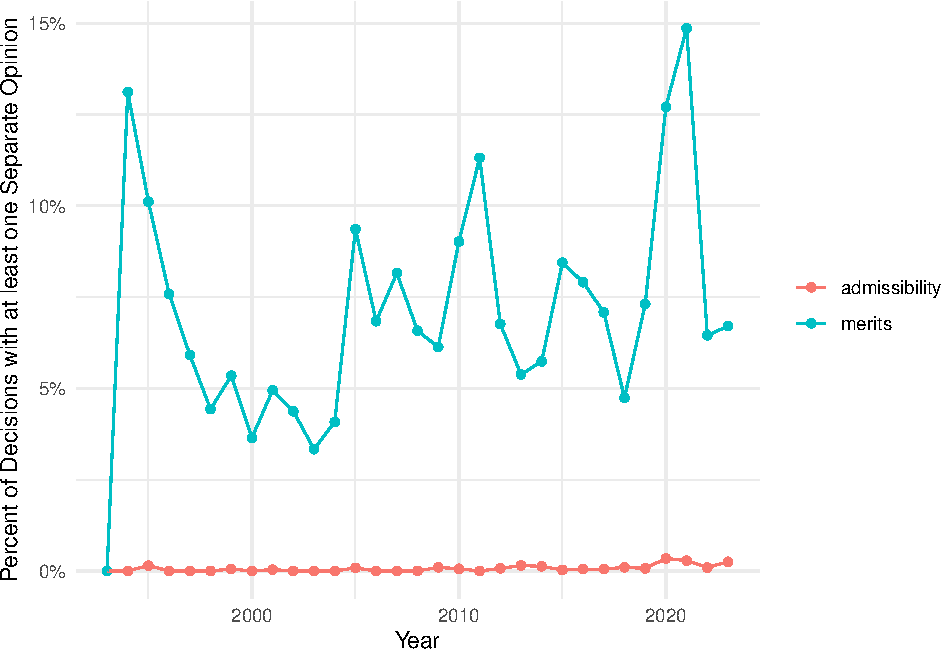
\includegraphics{separate_opinions_files/figure-latex/unnamed-chunk-1-1.pdf}
\caption{Percentage of Decisions with at least one Separate Opinion}
\end{figure}

We skip the first decade of the CCC as the data on it are rather
incomplete and inconsistent: For example, very few decisions contain the
information on the composition in the text and many do not contain the
name of the dissenting judge at all. We also limit our analysis until
the end of 2022 as the CCC entered its 4th term in 2023 and started to
undergo a complete personal change.

The final dataset for analysis contains 4668 decisions of the CCC. Out
of them, 81.2\% are decisions by the 3-member chambers on merits, around
9.2\% are plenum decisions on merits and the remaining 9.6\% are plenum
decisions on admissibility. At least one separate opinion contain 4.3\%
decisions out of the 3-member decisions, 11.2\% decisions of the plenum
decisionson admissibility, and 39.4\% decisions of the plenum decisions
on merits.

\begin{longtable}[t]{llrll}
\caption{\label{tab:unnamed-chunk-2}Summary statistics for the whole dataset}\\
\toprule
\textbf{Formation} & \textbf{Admissibility} & \textbf{Count} & \textbf{Ratio - Total} & \textbf{Dissents - Ratio}\\
\midrule
Chamber & merits & 3862 & 81.2\% & 4.3\%\\
Plenum & admissibility & 456 & 9.6\% & 11.2\%\\
Plenum & merits & 436 & 9.2\% & 39.4\%\\
\bottomrule
\end{longtable}

\hypertarget{operationalization}{%
\subsection{Operationalization}\label{operationalization}}

\hypertarget{dependent-variable-a-separate-opinion}{%
\subsubsection{Dependent variable: a separate
opinion}\label{dependent-variable-a-separate-opinion}}

We conceptualize our dependent variable as the information whether a
justice attached a separate opinion to a decision or not.\footnote{Unlike
  Wittig we do not call our dependent variable a judge's vote, as that
  refers to a slightly different thing within the CCC context. A judge
  may vote against the majority opinion but since they are not mandated
  to write a separate opinion, these do not necessarily overlap.
  Similarly, a judge may vote for a disposition of a case and still
  attach a concurrence separate opinion.} Our dependent variable
\emph{Separate opinion} is thus a dummy variable that has two
categories: either a justice did attach a separate opinion (1) or she
did not in any given case (0).

We do not distinguish between a concurrence and a dissent. The reason is
two-fold: practical and theoretical. Theoretically, the difference
between the two lays only in the disposition of the case. The justices
may equally disagree on the interpretation of legal rules, thus, in the
case-space model terms
(\protect\hyperlink{ref-landaDisagreementsCollegialCourts2007}{Landa and
Lax 2007--2008}; \protect\hyperlink{ref-laxNewJudicialPolitics2011}{Lax
2011}), the judge cut points in any given case differ even when a
justice attaches ``only'' concurrence. The difference is that in the
cases containing concurrence, the case facts may have completely
accidentally fallen on the same side both of the concurring judge as
well as the majority, whereas in the cases containing a dissenting
opinion, the case fell in between the cut points. We do not consider
this phenomenon as theoretically interesting. Practically, it was
impossible to distinguish between the two categories as some decisions
simply do not contain the information whether a separate opinion was a
concurring or dissenting opinion.

\hypertarget{explanatory-variables}{%
\subsubsection{Explanatory variables}\label{explanatory-variables}}

\hypertarget{disagreement-potential}{%
\paragraph{Disagreement potential}\label{disagreement-potential}}

From the theoretical perspective it may be expected that the potential
for disagreement varies across cases. In some cases, the disagreement
potential is higher and, thus, the likelihood of a separate opinion is
higher than in the cases with lower potential for disagreement. More
specifically, we expect the potential for disagreement to be captured by
two characteristics of any given case: (1) its complexity and (2) its
controversy.

\hypertarget{complexity}{%
\subparagraph{Complexity}\label{complexity}}

As Corley, Steigerwalt, and Ward
(\protect\hyperlink{ref-corleyPuzzleUnanimityConsensus2013}{2013}), p70
argue and empirically measure, complexity of a case leads to less
certainty and more ambiguity for the justices, which leads to a higher
likelihood of disagreement. The authors define legal complexity as the
number of legal issues a case has to address. True to the Corley,
Steigerwalt, and Ward
(\protect\hyperlink{ref-corleyPuzzleUnanimityConsensus2013}{2013})
study, our operationalization of complexity relies on the assumption
that the more legal issues there are in any given case, the higher the
number of references to other laws and caselaw in the text of the
corresponding decision.

The variable \emph{concerned acts} captures the number of concerned
ordinary legal acts on the legal-act level, the variable \emph{concerned
constitutional acts} captures the number of articles of the
constitutional legal acts (mostly the Czech Constitution and the Charter
of Fundamental Rights and Freedoms) and variable \emph{caselaw} captures
the number of citations to its own caselaw. The information on the first
two variables is based on the metadata provided by the CCC, the last is
based on the regular expressions search of the text of the decisions.

\begin{longtable}[t]{llll}
\caption{\label{tab:unnamed-chunk-3}Correlations between Independent Variables of Case Complexity}\\
\toprule
\textbf{Variable} & \textbf{1} & \textbf{2} & \textbf{3}\\
\midrule
1. \# of Ordinary Acts & — & — & —\\
2. \# of Constitutional Articles & .35 & — & —\\
3. \# of CCC References & .32 & .48 & —\\
\bottomrule
\multicolumn{4}{l}{\rule{0pt}{1em}\textit{Note.} Correlation was calculated using the Spearman Correlation Coefficient.}\\
\end{longtable}

The first two we believe to be sufficiently different from each other: a
typical right to fair proceedings case may concern only one
constitutional article (the article 36 of the Charter) but many legal
acts, whereas a typical separation of powers case concerning the
Parliament concerns many consitutional articles but only few ordinary
laws. On the other hand, the number of (concerned) constitutional acts
and references to the CCC caselaw may be correlated. We therefore run
diagnostics, which reveal that the citations to CCC caselaw and the
number of references to constitutional acts are rather correlated.
Because we believe the number of cited constitutional articles to better
reflect the number of legal issues than the number of references to CCC
case-law, we stick only to that variable.

\hypertarget{controversy}{%
\subparagraph{Controversy}\label{controversy}}

In a similar vein, certain typically value-laden topics may generate
more disagreement even if they raise only one or few legal questions.
Typically, the restitution cases or cases concerning fundamental human
rights have been coined as rather controversial. The CCC dataset
contains a variable \emph{subject\_proceedings}, which contains the
subject matter of any given case (a discrimination case, a separation of
powers case and alike), and a variable \emph{field\_register}, which
refers to the area of constitutional law that the case pertains (the
right to fair trial, the right of freedom of speech).

We coded the topics as controversial when they concern any of the
following subject matters or areas of constitutional law:
discrimination, expropriation, restitution, the property of church,
sexual orientation, the protection of consumer, fundamental human
rights, social and cultural rights, the right of property, the freedom
of speech, and the separation between the church and state. Therefore,
the variable \emph{controversial} is a dummy variable, which takes the
value of 1 when the given case falls in any of the previously mentioned
categories or it takes the value 0 when it does not.

\hypertarget{norm-identification}{%
\paragraph{Norm-identification}\label{norm-identification}}

Secondly, our theory generated a second expectation: a relationship
between adherence to norm of consensus and one's career choices.
Theoretically, the actors socialized within the judiciary and its values
are more likely to adhere to them than their peers who entered the CCC
from the legal practice
(\protect\hyperlink{ref-wittigOccurrenceSeparateOpinions2016}{Wittig
2016, 84--87}.). Wittig confirms this intuition also empirically.

Wittig thus operationalizes the norm-identification as the justices'
career choice after their term. The justices that chose to stay within
judiciary or go back to being scholars are expected to more strongly
identify with the norm of consensus, whereas the justices' that made
different career choice are less likely to identify with the norm of
consensus.

\begin{figure}
\centering
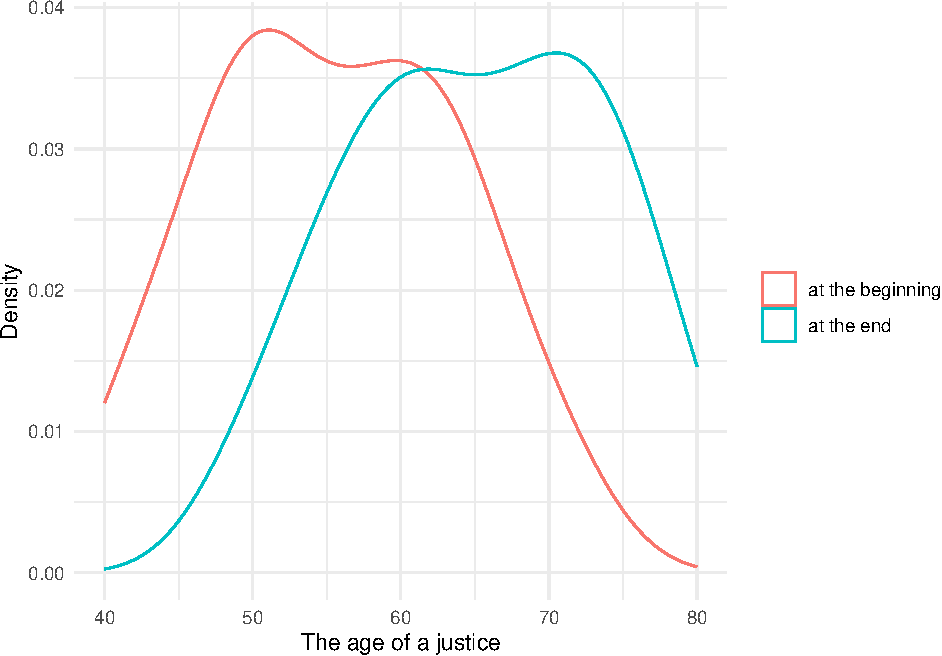
\includegraphics{separate_opinions_files/figure-latex/unnamed-chunk-4-1.pdf}
\caption{Kernel density of justices' ages at the start and and the end
of their terms}
\end{figure}

Unfortunately, such a measure does not fit the CCC context. As the data
shows, CCC justices start their term usually at the end of their career
and a considerable part of them ends their term in their 70s, well past
the retirement age in Czechia. Therefore, instead of operationalizing
the norm-identification as the profession after their term, we
operationalize it as the profession before they entered the CCC. Quite
handily, the CCC dataset contains such an information on the last
profession before the CCC justices took up their office.

The variable \emph{profession} contains the information on the justices'
previous career choices and can take up the values of judge, scholar,
politician, or lawyer. We can observe that the distribution of the
professions has changed across time. While the 1st and 2nd terms of the
CCC were quite balanced in terms of the professions, its 3rd term is
heavily skewed towards the more to the norm of consensus adherent
professions.

\begin{figure}
\centering
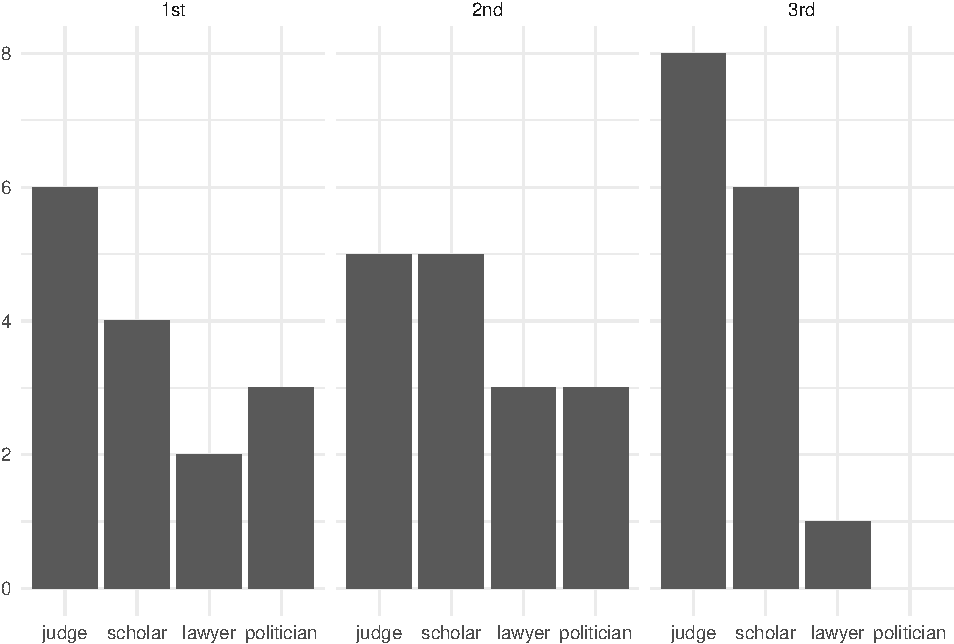
\includegraphics{separate_opinions_files/figure-latex/unnamed-chunk-5-1.pdf}
\caption{The distribution of professions of the CCC justices across its
3 terms.}
\end{figure}

\hypertarget{time-in-office}{%
\paragraph{Time in office}\label{time-in-office}}

The effects of the CCC justices' profession should according to our
theoretical expectations vary depending on the time the judges have
spent in their office. The closer to them taking up the office, the
effects of their preceding profession should be more pronounced.
Similarly, according to the collegiality costs hypothesis, the
dissenting behavior of justices should vary across time. Namely,
justices are expected to dissent less at the beginning of their terms,
as the collegiality costs are higher, and to dissent more at the end of
their terms, as the collegiality costs of the disagreement are lower. We
capture the \emph{time in office} variables as the number of months a
justice has left until their end of mandate from the date of decision.
That allows us to account both for the collegiality costs hypothesis as
well as the difference between professions hypothesis.

\hypertarget{workload}{%
\paragraph{Workload}\label{workload}}

Similarly to Brekke, Naurin, et al.
(\protect\hyperlink{ref-brekkeThatOrderHow2023}{2023}), we
operationalize \emph{workload} as the number of pending unfinished cases
that any given judge has in the moment of any given decision as a judge
rapporteur. We firstly mined the compositions of panels as well as the
plenary from the text of the decision. We then calculated the number of
unfinished cases each judge had at the time of any given decision as a
judge rapporteur using the date of submission and of decision of a case.

To address potential sources of bias in our regression analysis, we
consider the workload of a judge to be assigned as good as random. The
cases once submitted to the CCC get assigned to individual judges
rapoprteurs based on the alphabetic order of their surnames. There is no
intentional case selection in play. Therefore the assignment of cases to
judges is independent of other covariates and so is the outcome of
interest.

\hypertarget{control-variables}{%
\subsubsection{Control Variables}\label{control-variables}}

Lastly, we control for multiple potential confounding variables. A
confounding variable is such that (1) has an effect on treatment status
and (2) has an effect on the outcome over and above its effect on the
treatment status. Not controlling for confounding variables causes an
omitted variable bias
(\protect\hyperlink{ref-angristMostlyHarmlessEconometrics2009}{Angrist
and Pischke 2009},
\protect\hyperlink{ref-angristMasteringMetricsPath2014}{2014};
\protect\hyperlink{ref-buenodemesquitaThinkingClearlyData2021}{Bueno de
Mesquita and Fowler 2021}). Therefore, we need to carefully consider
which additional features may induce bias rather than throw in as many
additional variables as possible.

\hypertarget{identification-strategy}{%
\subsection{Identification Strategy}\label{identification-strategy}}

The hypotheses are tested by fitting a generalized linear model
estimating the probability of a judge attaching a separate opinion with
the dependent variable following a binomial distribution.

When identifying our model, we stood before a research choice that has
been addressed differently by different researchers. As other studies on
judicial decision-making relying on observational data, the data on
judicial-decision making offers multiple potential clustering variables
to fix effects. In their study of effect of french language on the
performance of the judges at the CJEU, Cheruvu
(\protect\hyperlink{ref-cheruvuHowInstitutionalConstraints2019}{2019})
fixed in their model the effects both on the individual judges as well
as on the panel level. The reasoning behind fixed effects clustered on
the formation were that it ``{[}s{]}cholars argue the number of judges
sitting on a chamber is a proxy for a cases' salience as more important
cases tend to be assigned to larger chambers (e.g.~Kelemen, 2012;
Larsson and Naurin, 2016). Including chamber fixed-effects in my models
addresses both heterogeneity in the collegial decisionmaking process of
different chambers of judges and implicitly controls for the number of
judges hearing a case.'' In a similar study, in which Clark, Engst, and
Staton (\protect\hyperlink{ref-clarkEstimatingEffectLeisure2018}{2018})
studied the effect of leisure on judicial performance.\footnote{Also
  measured as time for a judge to decide a case similarly to the Cheruvu
  (\protect\hyperlink{ref-cheruvuHowInstitutionalConstraints2019}{2019})
  study.}, in which the the author fixed effects were included in the
model.\footnote{Which would correspond to the judge rapporteur in our
  case.} Brekke, Fjelstul, et al.
(\protect\hyperlink{ref-brekkeCJEUDatabasePlatform2023}{2023}) in a
study on the usage of orders at the CJEU built a logistic regression
model with subject matter fixed effects.

\hypertarget{results}{%
\subsection{Results}\label{results}}

The results reveal quite an interesting trend at the CCC. Standard
errors are clustered at the level of the unique combination of three
judges deciding each case (that is, the panel) to avoid any downward
bias in uncertainty that might result from different numbers of
observations from the circuits.

\begin{table}
\centering
\caption{\label{tab:unnamed-chunk-6}Results from the Logit Model}
\centering
\begin{tabular}[t]{lc}
\toprule
  & (1)\\
\midrule
(Intercept) & \num{-3.678}***\\
 & (\num{0.168})\\
n\_concerned\_acts & \num{0.052}***\\
 & (\num{0.009})\\
n\_concerned\_constitutional\_acts & \num{0.112}***\\
 & (\num{0.010})\\
n\_citations & \num{0.031}***\\
 & (\num{0.003})\\
merits\_admissibilitymerits & \num{-0.212}*\\
 & (\num{0.105})\\
judge\_professionlawyer & \num{-0.257}\\
 & (\num{0.260})\\
judge\_professionpolitician & \num{0.650}*\\
 & (\num{0.273})\\
judge\_professionscholar & \num{0.323}*\\
 & (\num{0.154})\\
time\_in\_office & \num{-0.003}+\\
 & \vphantom{1} (\num{0.002})\\
controversial & \num{0.635}***\\
 & (\num{0.114})\\
workload & \num{-0.003}***\\
 & (\num{0.001})\\
judge\_professionlawyer × time\_in\_office & \num{0.003}\\
 & \vphantom{1} (\num{0.004})\\
judge\_professionpolitician × time\_in\_office & \num{-0.014}**\\
 & (\num{0.004})\\
judge\_professionscholar × time\_in\_office & \num{0.001}\\
 & (\num{0.002})\\
\midrule
Num.Obs. & \num{21741}\\
AIC & \num{6670.2}\\
BIC & \num{6782.0}\\
Log.Lik. & \num{-3321.075}\\
F & \num{56.183}\\
RMSE & \num{0.19}\\
\bottomrule
\end{tabular}
\end{table}

\hypertarget{conclusions}{%
\section{Conclusions}\label{conclusions}}

\vspace{30pt}

\hypertarget{literature}{%
\section*{Literature}\label{literature}}
\addcontentsline{toc}{section}{Literature}

\hypertarget{refs}{}
\begin{CSLReferences}{1}{0}
\leavevmode\vadjust pre{\hypertarget{ref-angristMostlyHarmlessEconometrics2009}{}}%
Angrist, Joshua D., and Jörn-Steffen Pischke. 2009. \emph{Mostly
{Harmless Econometrics}: {An Empiricist}'s {Companion}}. {Princeton
University Press}. \url{https://books.google.com?id=YSAzEAAAQBAJ}.

\leavevmode\vadjust pre{\hypertarget{ref-angristMasteringMetricsPath2014}{}}%
---------. 2014. \emph{Mastering '{Metrics}: {The Path} from {Cause} to
{Effect}}. {Princeton University Press}.

\leavevmode\vadjust pre{\hypertarget{ref-arnoldScalingCourtDecisions2023}{}}%
Arnold, Christian, Benjamin G. Engst, and Thomas Gschwend. 2023.
{``Scaling {Court Decisions} with {Citation Networks}.''} \emph{Journal
of Law and Courts} 11 (1): 25--44. \url{https://doi.org/10.1086/717420}.

\leavevmode\vadjust pre{\hypertarget{ref-berdejoElectoralCyclesUS2017}{}}%
Berdejó, Carlos, and Daniel L. Chen. 2017. {``Electoral {Cycles} Among
{US Courts} of {Appeals Judges}.''} \emph{The Journal of Law and
Economics} 60 (3): 479--96. \url{https://doi.org/10.1086/696237}.

\leavevmode\vadjust pre{\hypertarget{ref-bielenBacklogsLitigationRates2018}{}}%
Bielen, Samantha, Ludo Peeters, Wim Marneffe, and Lode Vereeck. 2018.
{``Backlogs and Litigation Rates: {Testing} Congestion Equilibrium
Across {European} Judiciaries.''} \emph{International Review of Law and
Economics} 53 (March): 9--22.
\url{https://doi.org/10.1016/j.irle.2017.09.002}.

\leavevmode\vadjust pre{\hypertarget{ref-boydUntanglingCausalEffects2010}{}}%
Boyd, Christina L., Lee Epstein, and Andrew D. Martin. 2010.
{``Untangling the {Causal Effects} of {Sex} on {Judging}.''}
\emph{American Journal of Political Science} 54 (2): 389--411.
\url{https://www.jstor.org/stable/25652213}.

\leavevmode\vadjust pre{\hypertarget{ref-brekkeCJEUDatabasePlatform2023}{}}%
Brekke, Stein Arne, Joshua C. Fjelstul, Silje Synnøve Lyder Hermansen,
and Daniel Naurin. 2023. {``The {CJEU Database Platform}: {Decisions}
and {Decision-Makers}.''} \emph{Journal of Law and Courts}, January,
1--22. \url{https://doi.org/10.1017/jlc.2022.3}.

\leavevmode\vadjust pre{\hypertarget{ref-brekkeThatOrderHow2023}{}}%
Brekke, Stein Arne, Daniel Naurin, Urška Šadl, and Lucía López-Zurita.
2023. {``That's an {Order}! {How} the {Quest} for {Efficiency Is
Transforming Judicial Cooperation} in {Europe}.''} \emph{JCMS: Journal
of Common Market Studies} 61 (1): 58--75.
\url{https://doi.org/10.1111/jcms.13346}.

\leavevmode\vadjust pre{\hypertarget{ref-buenodemesquitaThinkingClearlyData2021}{}}%
Bueno de Mesquita, Ethan, and Anthony Fowler, eds. 2021. \emph{Thinking
Clearly with Data: A Guide to Quantitative Reasoning and Analysis}. 1st.
edition. {Princeton}: {Princeton University Press}.

\leavevmode\vadjust pre{\hypertarget{ref-calderiaTimeConsensualNorms1998}{}}%
Calderia, Gregory A., and Christopher J. W. Zorn. 1998. {``Of {Time} and
{Consensual Norms} in the {Supreme Court}.''} \emph{American Journal of
Political Science} 42 (3): 874--902.
\url{https://doi.org/10.2307/2991733}.

\leavevmode\vadjust pre{\hypertarget{ref-cameronChapterWhatJudges2017}{}}%
Cameron, Charles M., and Lewis A. Kornhauser. 2017. {``Chapter 3: {What
Do Judges Want}? {How} to {Model Judicial Preferences}.''} SSRN
Scholarly Paper. {Rochester, NY}. June 2, 2017.
\url{https://doi.org/10.2139/ssrn.2979419}.

\leavevmode\vadjust pre{\hypertarget{ref-carrubbaWhoControlsContent2012}{}}%
Carrubba, Cliff, Barry Friedman, Andrew D. Martin, and Georg Vanberg.
2012. {``Who {Controls} the {Content} of {Supreme Court Opinions}?''}
\emph{American Journal of Political Science} 56 (2): 400--412.
\url{https://doi.org/10.1111/j.1540-5907.2011.00557.x}.

\leavevmode\vadjust pre{\hypertarget{ref-cheruvuHowInstitutionalConstraints2019}{}}%
Cheruvu, Sivaram. 2019. {``How Do Institutional Constraints Affect
Judicial Decision-Making? {The European Court} of {Justice}'s {French}
Language Mandate.''} \emph{European Union Politics} 20 (4): 562--83.
\url{https://doi.org/10.1177/1465116519859428}.

\leavevmode\vadjust pre{\hypertarget{ref-chmelZpravodajoveSenatyVliv2017}{}}%
Chmel, Jan. 2017. {``Zpravodajové a Senáty: {Vliv} Složení Senátu Na
Rozhodování {Ústavního} Soudu {České} Republiky o Ústavních
Stížnostech.''} \emph{Časopis Pro Právní Vědu a Praxi} 25 (4): 739.
\url{https://doi.org/10.5817/CPVP2017-4-9}.

\leavevmode\vadjust pre{\hypertarget{ref-chmelCoOvlivnujeUstavni2021}{}}%
---------. 2021. \emph{Co Ovlivňuje {Ústavní} Soud a Jeho Soudce? /}.
Vydání první. Teoretik ({Leges}). {Leges,}.

\leavevmode\vadjust pre{\hypertarget{ref-clarkEstimatingEffectLeisure2018}{}}%
Clark, Tom S., Benjamin G. Engst, and Jeffrey K. Staton. 2018.
{``Estimating the {Effect} of {Leisure} on {Judicial Performance}.''}
\emph{The Journal of Legal Studies} 47 (2): 349--90.
\url{https://doi.org/10.1086/699150}.

\leavevmode\vadjust pre{\hypertarget{ref-clarkLocatingSupremeCourt2010}{}}%
Clark, Tom S., and Benjamin Lauderdale. 2010. {``Locating {Supreme Court
Opinions} in {Doctrine Space}.''} \emph{American Journal of Political
Science} 54 (4): 871--90.
\url{https://doi.org/10.1111/j.1540-5907.2010.00470.x}.

\leavevmode\vadjust pre{\hypertarget{ref-corleyPuzzleUnanimityConsensus2013}{}}%
Corley, Pamela C., Amy Steigerwalt, and Artemus Ward. 2013. \emph{The
{Puzzle} of {Unanimity}: {Consensus} on the {United States Supreme
Court}}. {Redwood City, UNITED STATES}: {Stanford University Press}.
\url{http://ebookcentral.proquest.com/lib/huberlin-ebooks/detail.action?docID=1180198}.

\leavevmode\vadjust pre{\hypertarget{ref-coupetteQuantitativeRechtswissenschaft2018}{}}%
Coupette, Corinna, and Andreas M. Fleckner. 2018. {``Quantitative
{Rechtswissenschaft}.''} \emph{JuristenZeitung (JZ)} 73 (8): 379--89.
\url{https://doi.org/10.1628/jz-2018-0020}.

\leavevmode\vadjust pre{\hypertarget{ref-dworkinPoliticalJudgesRule1980}{}}%
Dworkin, Ronald M. 1980. \emph{Political Judges and the Rule of Law}.
{London}: {British Academy}.

\leavevmode\vadjust pre{\hypertarget{ref-engstEinflussParteinaheAuf2017}{}}%
Engst, Benjamin G., Thomas Gschwend, Nils Schaks, Sebastian Sternberg,
and Caroline Wittig. 2017. {``Zum {Einfluss} Der {Parteinähe} Auf Das
{Abstimmungsverhalten} Der {Bundesverfassungsrichter} -- Eine
Quantitative {Untersuchung}.''} \emph{JuristenZeitung} 72 (17): 816--26.
\url{https://www.jstor.org/stable/44867374}.

\leavevmode\vadjust pre{\hypertarget{ref-epsteinChoicesJusticesMake1997}{}}%
Epstein, Lee, and Jack Knight. 1997. \emph{The {Choices Justices Make}}.
{SAGE}. \url{https://books.google.com?id=hSnom2h2_zUC}.

\leavevmode\vadjust pre{\hypertarget{ref-epsteinStrategicRevolutionJudicial2000}{}}%
---------. 2000. {``Toward a {Strategic Revolution} in {Judicial
Politics}: {A Look Back}, {A Look Ahead}.''} \emph{Political Research
Quarterly} 53 (3): 625--61.
\url{https://doi.org/10.1177/106591290005300309}.

\leavevmode\vadjust pre{\hypertarget{ref-epsteinWhyWhenJudges2011}{}}%
Epstein, Lee, William M. Landes, and Richard A. Posner. 2011. {``Why
({And When}) {Judges Dissent}: {A Theoretical And Empirical
Analysis}.''} \emph{Journal of Legal Analysis} 3 (1): 101--37.
\url{https://doi.org/10.1093/jla/3.1.101}.

\leavevmode\vadjust pre{\hypertarget{ref-fjelstulEvolutionEuropeanUnion2019}{}}%
Fjelstul, Joshua C. 2019. {``The Evolution of {European Union} Law: {A}
New Data Set on the {\emph{Acquis Communautaire}}.''} \emph{European
Union Politics} 20 (4): 670--91.
\url{https://doi.org/10.1177/1465116519842947}.

\leavevmode\vadjust pre{\hypertarget{ref-fjelstulHowChamberSystem2023}{}}%
---------. 2023. {``How the {Chamber System} at the {CJEU Undermines}
the {Consistency} of the {Court}'s {Application} of {EU Law}.''}
\emph{Journal of Law and Courts}, 717422.
\url{https://doi.org/10.1086/717422}.

\leavevmode\vadjust pre{\hypertarget{ref-fjelstulTimelyAdministrationJustice2022}{}}%
Fjelstul, Joshua C., Matthew Gabel, and Clifford J. Carrubba. 2022.
{``The Timely Administration of Justice: Using Computational Simulations
to Evaluate Institutional Reforms at the {CJEU}.''} \emph{Journal of
European Public Policy}, August, 1--22.
\url{https://doi.org/10.1080/13501763.2022.2113115}.

\leavevmode\vadjust pre{\hypertarget{ref-foxallWhatJudgesMaximize2004}{}}%
Foxall, Gordon R. 2004. {``What Judges Maximize:toward an Economic
Psychology of the Judicial Utility Function.''} \emph{Liverpool Law
Review} 25 (3): 177--94.
\url{https://doi.org/10.1007/s10991-004-2877-9}.

\leavevmode\vadjust pre{\hypertarget{ref-gschwendAreJudgesPolitical2016}{}}%
Gschwend, Thomas, Sebastian Sternberg, and Steffen Zittlau. 2016. {``Are
{Judges Political Animals} After {All}? {Quasi-Experimental Evidence}
from the {German Federal Constitutional Court}.''} SSRN Scholarly Paper.
{Rochester, NY}. February 26, 2016.
\url{https://doi.org/10.2139/ssrn.2738512}.

\leavevmode\vadjust pre{\hypertarget{ref-hamannGermanFederalCourts2019}{}}%
Hamann, Hanjo. 2019. {``The {German Federal Courts Dataset} 1950--2019:
{From Paper Archives} to {Linked Open Data}.''} \emph{Journal of
Empirical Legal Studies} 16 (3): 671--88.
\url{https://doi.org/10.1111/jels.12230}.

\leavevmode\vadjust pre{\hypertarget{ref-hanrettyDissentIberiaIdeal2012}{}}%
Hanretty, Chris. 2012. {``Dissent in {Iberia}: {The} Ideal Points of
Justices on the {Spanish} and {Portuguese Constitutional Tribunals}.''}
\emph{European Journal of Political Research} 51 (5): 671--92.
\url{https://doi.org/10.1111/j.1475-6765.2012.02056.x}.

\leavevmode\vadjust pre{\hypertarget{ref-hanrettyCourtSpecialistsJudicial2020}{}}%
---------. 2020. \emph{A {Court} of {Specialists}: {Judicial Behavior}
on the {UK Supreme Court}}. {Oxford University Press}.
\url{https://doi.org/10.1093/oso/9780197509234.001.0001}.

\leavevmode\vadjust pre{\hypertarget{ref-horenovskyProcessMakingConstitutional2015}{}}%
Hořeňovský, Jan, and Jan Chmel. 2015. {``The Process of making the
Constitutional Court Judgements.''} \emph{Časopis pro právní vědu a
praxi} 23 (3): 302--11.
\url{https://www.ceeol.com/search/article-detail?id=780150}.

\leavevmode\vadjust pre{\hypertarget{ref-kastellecEmpiricallyEvaluatingCountermajoritarian2016}{}}%
Kastellec, Jonathan P. 2016. {``Empirically {Evaluating} the
{Countermajoritarian Difficulty}: {Public Opinion}, {State Policy}, and
{Judicial Review} Before {\emph{Roe}}{ \emph{v.} }{\emph{Wade}}.''}
\emph{Journal of Law and Courts} 4 (1): 1--42.
\url{https://doi.org/10.1086/683466}.

\leavevmode\vadjust pre{\hypertarget{ref-kornhauserModelingCollegialCourts1992a}{}}%
Kornhauser, Lewis A. 1992a. {``Modeling {Collegial Courts}. {II}. {Legal
Doctrine}.''} \emph{Journal of Law, Economics and Organization} 8: 441.
\url{https://heinonline.org/HOL/Page?handle=hein.journals/jleo8&id=449&div=&collection=}.

\leavevmode\vadjust pre{\hypertarget{ref-kornhauserModelingCollegialCourts1992}{}}%
---------. 1992b. {``Modeling Collegial Courts {I}:
{Path-dependence}.''} \emph{International Review of Law and Economics}
12 (2): 169--85. \url{https://doi.org/10.1016/0144-8188(92)90034-O}.

\leavevmode\vadjust pre{\hypertarget{ref-kosarConstitutionalCourtCzechia2020}{}}%
Kosař, David, and Ladislav Vyhnánek. 2020. {``The {Constitutional Court}
of {Czechia}.''} In \emph{The {Max Planck Handbooks} in {European Public
Law}: {Volume III}: {Constitutional Adjudication}: {Institutions}},
edited by Armin von Bogdandy, Peter Huber, and Christoph Grabenwarter,
0. {Oxford University Press}.
\url{https://doi.org/10.1093/oso/9780198726418.003.0004}.

\leavevmode\vadjust pre{\hypertarget{ref-landaDisagreementsCollegialCourts2007}{}}%
Landa, Dimitri, and Jeffrey R. Lax. 2007--2008. {``Disagreements on
{Collegial Courts}: {A Case-Space Approach}.''} \emph{University of
Pennsylvania Journal of Constitutional Law} 10: 305.
\url{https://heinonline.org/HOL/Page?handle=hein.journals/upjcl10&id=315&div=&collection=}.

\leavevmode\vadjust pre{\hypertarget{ref-lauderdaleScalingPoliticallyMeaningful2014}{}}%
Lauderdale, Benjamin E., and Tom S. Clark. 2014. {``Scaling {Politically
Meaningful Dimensions Using Texts} and {Votes}: {SCALING POLITICALLY
MEANINGFUL DIMENSIONS}.''} \emph{American Journal of Political Science}
58 (3): 754--71. \url{https://doi.org/10.1111/ajps.12085}.

\leavevmode\vadjust pre{\hypertarget{ref-laxNewJudicialPolitics2011}{}}%
Lax, Jeffrey R. 2011. {``The {New Judicial Politics} of {Legal
Doctrine}.''} \emph{Annual Review of Political Science} 14 (1): 131--57.
\url{https://doi.org/10.1146/annurev.polisci.042108.134842}.

\leavevmode\vadjust pre{\hypertarget{ref-moyerJudicialInnovationSexual2012}{}}%
Moyer, Laura P., and Holley Tankersley. 2012. {``Judicial {Innovation}
and {Sexual Harassment Doctrine} in the {U}.{S}. {Courts} of
{Appeals}.''} \emph{Political Research Quarterly} 65 (4): 784--98.
\url{https://doi.org/10.1177/1065912911411097}.

\leavevmode\vadjust pre{\hypertarget{ref-narayanConsensualNormHigh2005}{}}%
Narayan, Paresh Kumar, and Russell Smyth. 2005. {``The {Consensual Norm}
on the {High Court} of {Australia}: 1904-2001.''} \emph{International
Political Science Review} 26 (2): 147--68.
\url{https://doi.org/10.1177/0192512105050379}.

\leavevmode\vadjust pre{\hypertarget{ref-posnerWhatJudgesJustices1993}{}}%
Posner, Richard A. 1993. \emph{What {Do Judges} and {Justices
Maximize}?: (The {Same Thing Everyone Else Does})}. {Law School,
University of Chicago}. \url{https://books.google.com?id=ciFUHQAACAAJ}.

\leavevmode\vadjust pre{\hypertarget{ref-posnerHowJudgesThink2010}{}}%
---------. 2010. \emph{How {Judges Think}}. {Harvard University Press}.
\url{https://books.google.com?id=ZVUC8riEVPQC}.

\leavevmode\vadjust pre{\hypertarget{ref-rousseyOverburdenedJudges2018}{}}%
Roussey, Ludivine, and Raphael Soubeyran. 2018. {``Overburdened
Judges.''} \emph{International Review of Law and Economics} 55
(September): 21--32. \url{https://doi.org/10.1016/j.irle.2018.02.003}.

\leavevmode\vadjust pre{\hypertarget{ref-scaliaDissents1998}{}}%
Scalia, Antonin. 1998. {``Dissents.''} \emph{OAH Magazine of History} 13
(1): 18--23. \url{https://www.jstor.org/stable/25163249}.

\leavevmode\vadjust pre{\hypertarget{ref-smekalMimopravniVlivyNa2021}{}}%
Smekal, Hubert, Jaroslav Benák, Monika Hanych, Ladislav Vyhnánek, and
Štěpán Janků. 2021. \emph{Mimoprávní Vlivy Na Rozhodování Českého
{Ústavního} Soudu:} {Brno}: {Masaryk University Press}.
\url{https://doi.org/10.5817/CZ.MUNI.M210-9884-2021}.

\leavevmode\vadjust pre{\hypertarget{ref-sunsteinAreJudgesPolitical2006}{}}%
Sunstein, Cass R., David Schkade, Lisa M. Ellman, and Andres Sawicki.
2006. \emph{Are {Judges Political}? {An Empirical Analysis} of the
{Federal Judiciary}}. {Brookings Institution Press}.
\url{https://www.jstor.org/stable/10.7864/j.ctt12879t7}.

\leavevmode\vadjust pre{\hypertarget{ref-vartazaryanSitOvaAnalyza2022}{}}%
Vartazaryan, Gor. 2022. {``Sít'ová Analỳza Disentujících Ústavních
Soudců.''} \emph{Pravnik}, no. 12.

\leavevmode\vadjust pre{\hypertarget{ref-wittigOccurrenceSeparateOpinions2016}{}}%
Wittig, Caroline. 2016. \emph{The {Occurrence} of {Separate Opinions} at
the {Federal Constitutional Court}}. {Logos Verlag Berlin}.
\url{https://doi.org/10.30819/4411}.

\end{CSLReferences}

\end{document}
